\documentclass[10pt,pdf,hyperref={unicode}]{beamer}


\usepackage{xltxtra}

\usepackage{polyglossia}
\setmainlanguage{russian}
\setotherlanguage{english}
\setkeys{russian}{babelshorthands=true}

\setmainfont{Times New Roman}
\setromanfont{Times New Roman} 
\setsansfont{Arial} 
\setmonofont{Courier New} 

\newfontfamily{\cyrillicfont}{Times New Roman} 
\newfontfamily{\cyrillicfontrm}{Times New Roman}
\newfontfamily{\cyrillicfonttt}{Courier New}
\newfontfamily{\cyrillicfontsf}{Arial}

\addto\captionsrussian{%
  \renewcommand{\figurename}{Рис.}%
  \renewcommand{\tablename}{Табл.}%
}




%%% Оформление абзацев %%%
\usepackage{indentfirst}                            % Красная строка

%%% Цвета %%%

%%\usepackage[dvipsnames, table, hyperref]{xcolor} % Совместимо с tikz


%%% Таблицы %%%
\usepackage{longtable,ltcaption}                    % Длинные таблицы
\usepackage{multirow,makecell}                      % Улучшенное форматирование таблиц

%%% Общее форматирование
\usepackage{soulutf8}                               % Поддержка переносоустойчивых подчёркиваний и зачёркиваний
\usepackage{icomma}                                 % Запятая в десятичных дробях


%%% Гиперссылки %%%
%\usepackage{hyperref}[2012/11/06]

%%% Изображения %%%
\usepackage{graphicx}[2014/04/25]                   % Подключаем пакет работы с графикой

%%% Счётчики %%%
%\usepackage[figure,table]{totalcount}               % Счётчик рисунков и таблиц
%\usepackage{totcount}                               % Пакет создания счётчиков на основе последнего номера подсчитываемого элемента (может требовать дважды компилировать документ)
%\usepackage{totpages}                               % Счётчик страниц, совместимый с hyperref (ссылается на номер последней страницы). Желательно ставить последним пакетом в преамбуле


%\usepackage{cleveref} 


%% Векторная графика

\usepackage{tikz}                   % Продвинутый пакет векторной графики
\usetikzlibrary{chains}             % Для примера tikz рисунка
\usetikzlibrary{shapes.geometric}   % Для примера tikz рисунка
\usetikzlibrary{shapes.symbols}     % Для примера tikz рисунка
\usetikzlibrary{arrows}             % Для примера tikz рисунка


%%% Математические пакеты %%%
\usepackage{amsthm,amsmath,amscd}   % Математические дополнения от AMS
\usepackage{amsfonts,amssymb}       % Математические дополнения от AMS
\usepackage{mathtools}              % Добавляет окружение multlined

%%%% Установки для размера шрифта 14 pt %%%%
%% Формирование переменных и констант для сравнения (один раз для всех подключаемых файлов)%%
%% должно располагаться до вызова пакета fontspec или polyglossia, потому что они сбивают его работу
\newlength{\curtextsize}
\newlength{\bigtextsize}
\setlength{\bigtextsize}{13.9pt}


% тема оформления
\usetheme{Bergen}

% цветовая схема
\usecolortheme{orchid}


\title{Эконометрика и машинное обучение}   
\subtitle{Бишкек}
\author{Стефановский Д.В.} 
\date{\today} 
\logo{
\includegraphics[height=5mm]{images/logo.jpg}\vspace{14cm}}
\institute{РАНХиГСМНИИПУ}


\usepackage{textpos}

\def\insertauthorindicator{}% Default is "Who?"
\def\insertinstituteindicator{}% Default is "From?"
\def\insertdateindicator{}% Default is "When?"


\begin{document}

% титульный слайд
\begin{frame}
\titlepage
\end{frame} 

\begin{frame}
\frametitle{Предмет и методы эконометрики} 
\framesubtitle{История}

Эконометрика как наука возникла в первой половине 20-го века в результате 
активного использования для решения задач экономической теории математических и статистических методов.
Термин эконометрика введен в научную литературу в 1930 году норвежским статистиком Рагнаром Фришем. 
Он первым определил эконометрику, как научную дисциплину, 
базирующуюся на синтезе экономической теории, статистики и математики.

\end{frame}


\begin{frame}
\frametitle{Предмет и методы эконометрики} 
\framesubtitle{История}

Эконометрика как наука возникла в первой половине 20-го века в результате 
активного использования для решения задач экономической теории математических и статистических методов.
Термин эконометрика введен в научную литературу в 1930 году норвежским статистиком Рагнаром Фришем. 
Он первым определил эконометрику, как научную дисциплину, 
базирующуюся на синтезе экономической теории, статистики и математики.

\end{frame}





\begin{frame}
\frametitle{Предмет и методы эконометрики} 
\framesubtitle{Главная задача}

Основной задачей эконометрики является 
количественная оценка имеющихся взаимосвязей между 
экономическими явлениями и процессами.



\end{frame}



\begin{frame}
\frametitle{Предмет и методы эконометрики} 
\framesubtitle{Инструменты}

Для количественной оценки необходима модель для экономического процесса
основные  инструменты моделирования взяты из  математической статистики
в основном это методы корреляционного и
регрессионного анализа.
\end{frame}









\begin{frame}
\frametitle{Предмет и методы эконометрики} 
\framesubtitle{Инструменты}

Корреляционный анализ ставит своей целью проверку наличия и значимости 
линейной зависимости между переменными без разделения переменных на
зависимые и объясняющие. Ответ на эти вопросы дается с помощью вычисления 
показателей (коэффициентов) корреляции.
Регрессионный анализ направлен на выражение изучаемой зависимости в
виде аналитической формулы с предварительным выделением зависимых и
объясняющих переменных.

\end{frame}


\begin{frame}
\frametitle{Предмет и методы эконометрики} 
\framesubtitle{Этапы}

\begin{enumerate}
  \item  Постановка проблемы, т. е. определение цели и задач исследования, 
  выделение зависимых ($y_j$ ) и независимых ($x_k$ ) экономических переменных 
  на основе качественного анализа изучаемых взаимосвязей методами экономической теории.
  \item  Сбор необходимых исходных данных.
  \item  Построение эконометрической модели и оценка ее адекватности и степени соответствия исходным данным.
  \item  Использование модели для целей анализа и прогнозирования параметров исследуемого явления.
  \item  Качественная и количественная интерпретация полученных на основе
модели результатов.
  \item  Практическое использование результатов.
\end{enumerate}
\end{frame}


\begin{frame}
\frametitle{Предмет и методы эконометрики} 
\framesubtitle{Характеристика взаимосвязей}

Причинно-следственное отношение – это такая связь между явлениями,
при которой изменение одного из них, называемого причиной, ведет к изменению 
другого, называемого следствием. Следовательно, причина всегда предшествует следствию.
Причинно-следственные связи в социально-экономических явлениях обладают 
следующими особенностями. Во-первых, причина Х и следствие Y взаимодействуют 
не непосредственно, а через промежуточные факторы, которые,
как правило, при анализе опускаются. Формально это может быть выражено с
помощью схемы $X—>X'—>X''—>Y$, где $X'$ и $X''$ - промежуточные факторы.


\end{frame}


\begin{frame}
\frametitle{Предмет и методы эконометрики} 
\framesubtitle{Построение эконометрической модели}

Построение эконометрической модели начинается со спецификации модели, 
заключающейся в получении ответа на два вопроса: 

1) какие экономические
показатели (признаки) должны быть включены в модель; 

2) какой вид имеет аналитическая зависимость между отобранными признаками.


\end{frame}


\begin{frame}
\frametitle{Предмет и методы эконометрики} 
\framesubtitle{Построение эконометрической модели}

В обобщенной форме эконометрическая модель, описывающая взаимосвязи 
между явлениями или закономерности их развития, представляется с помощью соотношения:


$$ y=f(\alpha, x)+\epsilon, $$

где $f(\alpha ,x)$ – функционал, выражающий вид и структуру взаимосвязей. 
Величина y выражает уровень исследуемого явления и называется 
зависимой (объясняемой) переменной или результативным признаком; 
величина $x = (x_1, x_2 ,..., x_n)$ представляет собой 
вектор значений независимых (объясняющих) переменных $X$ или факторных признаков (факторов); 
через $α = ( \alpha_0 , \alpha_1 ,\alpha_2 ,..., \alpha_n )$ обозначен вектор некоторых произвольных констант, 
называемых параметрами модели; $\epsilon$ – ошибка модели.


\end{frame}


\begin{frame}
\frametitle{Предмет и методы эконометрики} 
\framesubtitle{Построение эконометрической модели}

$$ y=f(\alpha, x)+\epsilon, $$


Ошибка модели $\epsilon$ характеризует отличие наблюдаемого (реализованного)
значения переменной у от вычисленных согласно соотношения
в конкретных условиях (при конкретных значениях переменных факторов $x_i$ ) 
и рассматривается как случайная величина.

Для расчета численных значений параметров $ \alpha_0 , \alpha_1 ,\alpha_2 ,..., \alpha_n $
используется предварительно накопленный массив наблюдений за совместным проявлением
изучаемого процесса и рассматриваемых факторов. 
Одно наблюдение представляет собой множество значений $(y_t , x_{1t} , x_{2t} , ,..., x_{nt})$. 
Индекс $t$  соответствует отдельному наблюдению.

\end{frame}


\begin{frame}
\frametitle{Предмет и методы эконометрики} 
\framesubtitle{Три этапа построения эконометрической модели}

1. Спецификация модели, т. е. выбор класса моделей, наиболее 
подходящих для описания изучаемых явлений и процессов. 
Этот этап предполагает решение двух задач:

а) отбор существенных факторов для их последующего включения в модель;

б) выбор типа модели, т. е. выбор вида аналитической зависимости, 
связывающей включенные в модель переменные.

2. Оценка параметров модели, т. е. получение численных значений 
констант модели. При этом используется предварительно 
полученный массив исходных данных.

3. Проверка качества построенной модели и обоснование возможности ее
дальнейшего использования.

\end{frame}


\begin{frame}
\frametitle{Предмет и методы эконометрики} 
\framesubtitle{Примеры эконометрических моделей}

Производственная функция . Производственной функцией называется 
соотношение между входными факторами производства и выпуском продукции.
Производственная функция часто применяется для оценки эластичности 
выпуска продукции по отдельным факторам производства. 
Например, производственная функция Кобба-Дугласа имеет вид:

$$ P= a L^\alpha * K^{(1-\alpha)} $$

Р – выпуск продукции;

L – затраты труда;

K – объем капитала;

$$0<\alpha< 1.$$




\end{frame}



\begin{frame}
\frametitle{Предмет и методы эконометрики} 
\framesubtitle{Примеры эконометрических моделей}


$Y_t= C_t + I_t +G_t.$ (тождество дохода)

где $С_t$ – потребление;

$Y_t$ – ВВП;

$I_t$ – валовые инвестиции;

$G_t$ – государственные расходы;

$t$ – текущий период;

$t-1$ – предыдущий период.


\end{frame}





\begin{frame}
\frametitle{Регрессионный анализ} 
\framesubtitle{Парная регрессия}

Парной регрессией в теории вероятностей и математической статистике принято
называть зависимость среднего значения какой-либо величины ( y ) от некоторой
другой величины или от нескольких величин.
Парной регрессией называется модель, выражающая зависимость 
среднего значения зависимой переменной y 
от одной независимой переменной х
$$ y= f(x) ,$$

где у – зависимая переменная (результативный признак); х – независимая,
объясняющая переменная (признак–фактор).

\end{frame}

\begin{frame}
\frametitle{Регрессионный анализ} 
\framesubtitle{Множественная регрессия}

Множественной регрессией в теории вероятностей и математической статистике принято
называть зависимость среднего значения какой-либо величины ( y ) от некоторой
другой величины или от нескольких величин.
Парной регрессией называется модель, выражающая зависимость 
среднего значения зависимой переменной y 
от одной независимой переменной х
$$ y= f(x_1,x_2, x_3 .....x_m) ,$$

где у – зависимая переменная (результативный признак); $x_i$ – независимые,
объясняющие переменные (признак–фактор).

\end{frame}

\begin{frame}
\frametitle{Регрессионный анализ} 
\framesubtitle{Множественная регрессия}

Множественной регрессией в теории вероятностей и математической статистике принято
называть зависимость среднего значения какой-либо величины ( y ) от некоторой
другой величины или от нескольких величин.
Парной регрессией называется модель, выражающая зависимость 
среднего значения зависимой переменной y 
от одной независимой переменной х
$$ y= f(x_1,x_2, x_3 .....x_m) ,$$

где у – зависимая переменная (результативный признак); $x_i$ – независимые,
объясняющие переменные (признак–фактор).

\end{frame}

\begin{frame}
\frametitle{Регрессионный анализ} 
\framesubtitle{МНК}

Для оценки параметров  уравнения регрессии обычно пользуются
методом наименьших квадратов (МНК). При определенных предположениях
относительно ошибки $\epsilon$ МНК дает наилучшие оценки параметров линейной
модели, то  есть выбираются такие значения параметров, при которых
сумма квадратов отклонений фактических значений результативного признака
от расчитанных значений минимальна.

$$ \sum_{i=1}^n(\hat{y_i} -y_i)^2 \rightarrow min$$ 

$\hat{y_i}$ - измеренное(реальное) значение

$y_i$   -  расчитанной с учетом подобранных формул 


\end{frame}


\begin{frame}
\frametitle{Регрессионный анализ} 
\framesubtitle{Условия Гаусса-Маркова}
1. Математическое ожидание отклонений фактических значений результативного признака
от расчитанных значений  равно нулю . 
Это означает, что случайное отклонение не должно иметь систематического смещения.

2. Дисперсия отклонений постоянна. Выполнимость данной предпосылки называется гомоскедастичпостъю, а ее невыполнимость — гетероскедастичистью.

3.  Отклонения  не коррелируют между собой (отсутствует автокорреляция)

По мимо этих трех условий обычно предполагается, 
что случайное отклонение имеет нормальный закон распределения



\end{frame}



\begin{frame}
\frametitle{Регрессионный анализ} 
\framesubtitle{Проверка качества уравнения регрессии. F-критерий Фишера}

Введем следующие обозначения:

$TSS =\sum_{i=1}^n(y_i-\overline{y})^2 $  олная сумма квадратов отклонений;

$ESS =\sum_{i=1}^n(\hat{y_i}-\overline{y})^2 $ объясненная сумма квадратов отклонений;

$RSS =\sum_{i=1}^n(\hat{y_i} - y_i)^2 $ необъясненная сумма квадратов отклонений.

$ F=\frac{\frac{ESS}{k}}{\frac{RSS}{n-k-1}} $

где  n - число наблюдений, 

k - число независимых переменных в уравнении регрессии (для парной регрессии k = 1) 

Далее расчитывается уровень значимости (обозначается $\alpha$).
 Уровень значимости  обычно принимает значения 0,05 и 0,01, что соответствует вероятности 
 совершения ошибки первого рода 5 \% и 1 \%. Сегодня расчет автоматизирован 
 и  в большинстве случаев нет необходимости обращаться к таблицам Фишера.  


\end{frame}


\begin{frame}{Проблемы}

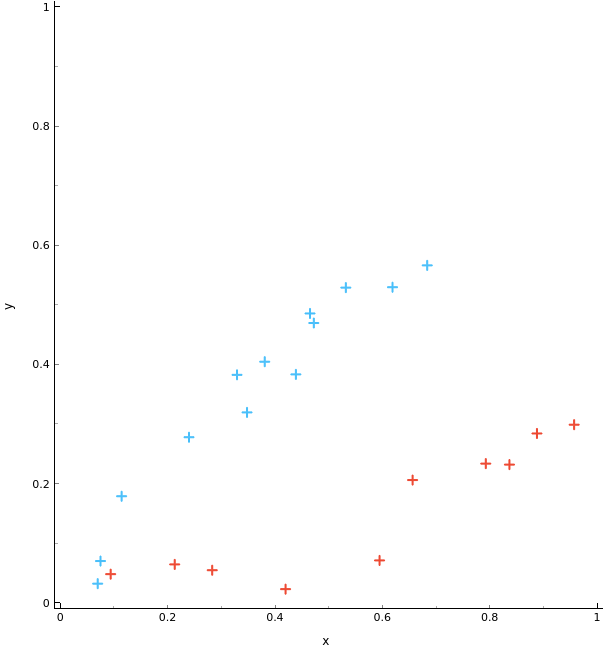
\includegraphics[scale=0.4]{images/problem.png}

Решить задачу на Orange3

\end{frame}


\begin{frame}{Проблемы}

Если  дисперсия случайного члена непостоянна, то в этом случае 
говорят о гетероскедастичности остатков, 
а сами остатки называются гетероскедастичными.  
Если наоборот  то можно говорить о  гомоскедастичности остатков.




\end{frame}

\begin{frame}{Проблемы}

Под мультиколлинеарностью понимается высокая взаимная коррелированность 
объясняющих переменных. Следствием мультиколлинеарности является 
линейная зависимость между столбцами наблюдений ($x_{ij}$). Это приводит к неустойчивости 
оценок коэффициентов регрессии, когда незначительные изменения данных 
наблюдений приводят к значительным изменениям оценок. 



\end{frame}


\begin{frame}
\frametitle{Регрессионный анализ} 
\framesubtitle{Другой подход}

 При определенных предположениях, о том что часть данных являются 
 выбросами можно записать несколько иную формулу:
 
$$ \sum_{i=1}^n \omega_i(\hat{y_i} -y_i)^2 \rightarrow min$$ 

$\hat{y_i}$ - измеренное(реальное) значение

$y_i$   -  расчитанной с учетом подобранных формул 

$\omega_i$ - коэффициент определяющий так называюмую значимость, чем он больше  тем значимей наблюдение с точки зрения
регрресси.  


\end{frame}



\begin{frame}

В широком понимании данные представляют собой факты, текст,
графики, картинки, звуки, аналоговые или цифровые видео-сегменты.
Данные могут быть получены в результате измерений, экспериментов,
арифметических и логических операций.

\end{frame}

\begin{frame}
Данные должны быть представлены в форме, пригодной для 
хранения, передачи и обработки. Иными словами, данные --
это необработанный материал, предоставляемый поставщиками данных и используемый
потребителями для формирования информации на основе данных.
\end{frame}

\begin{frame}
Набор данных  представляют в простом случае двухмерной таблицей, в которой 
строки это объекты, а столбцы это атрибуты или еще их называют измерения

Атрибут - свойство, характеризующее объект: цвет глаз человека,
температура воды и т.д. Атрибут также называют полем таблицы.
\end{frame}



\begin{frame}

\textbf{Адекватность информации } - это уровень соответствия образа, создаваемого с помощью информации, реальному объекту, процессу, явлению.
 
 От степени адекватности информации зависит правильность принятия решения.

Адекватность информации может выражаться в трех формах: синтаксической, семантической и прагматической.

\end{frame}

\begin{frame}{Синтаксическая адекватность}

\textbf{Синтаксическая адекватность} отображает формально-структурные характеристики информации, не затрагивая ее смыслового содержания. 
На синтаксическом уровне учитываются тип носителя и способ представления информации, 
скорость ее передачи и обработки, размеры кодов представления информации, 
надежность и точность преобразования этих кодов и т. д.

Информацию, рассматриваемую с таких позиций, обычно называют данными.

\end{frame}

\begin{frame}{Семантическая адекватность}

\textbf{Семантическая адекватность} определяет степень соответствия образа объекта самому объекту. 
Здесь учитывается смысловое содержание информации. На этом уровне анализируются сведения, отражаемые информацией, 
рассматриваются смысловые связи. 
Таким образом, семантическая адекватность проявляется при наличии единства информации и пользователя. 
Эта форма служит для формирования понятий и представлений, выявления смысла, содержания информации и ее обобщения.

\end{frame}

\begin{frame}{Прагматическая адекватность}

\textbf{Прагматическая адекватность} отражает соответствие информации цели управления, реализуемой на ее основе. 
Прагматические свойства информации проявляются при наличии единcтва информации, пользователя и цели управления. 
На этом уровне анализируются потребительские свойства информации, связанные с практическим использованием информации, 
с соответствием ее целевой функции деятельности системы.

\end{frame}

\begin{frame}{Информационный процесс}

\begin{small}

\begin{itemize}


  \item Поиск информации — это извлечение  информации  для сбора и хранения 

  \item Сбор информации предназначен для придания информации адекватности.  Для этого необходима обработка информации, то есть
   преобразование информации из одного вида в другой, осуществляемое по формальным правилам. 
 
  \item Хранение информации — это способ распространения информации в пространстве и времени в доступном виде. Другая цель это  многократное
   использование информация. 

  \item  Передача. В процессе передачи информации обязательно участвуют источник и приемник информации: первый передает информацию, второй ее получает. Между ними действует 
  канал передачи информации — канал связи. 
 
\end{itemize}

\end{small}

\end{frame}








\begin{frame}{Типы данных:time-series} 

Временной ряд — совокупность наблюдений одного и того же показателя в различные моменты времени 
(обычно последовательные: дни, недели, месяцы, кварталы, годы и т.д.).

Показатели: цены акций, уровень безработицы, обменный курс евро/рубль и т.д. 
Характерной особенностью временных рядов является естественным образом зафиксированный порядок наблюдений. 


\end{frame}




\begin{frame}{Типы данных:cross-section}

''Перекрёстные данные'' — это тип данных, собранный путем наблюдения за многими объектами 
(такими как физические лица, фирмы, страны или регионы) в один и тот же период времени.

Для перекрестных данных (дословный перевод термина cross-sectional data, 
иногда он переводится как «пространственные данные» в противопоставление временным, или «временной срез») 
момент времени зафиксирован, и имеются наблюдения для различных однородных объектов (в этот момент). 
\end{frame}

\begin{frame}{Типы данных:panel-data} 

Панельные данные —  это набор наблюдений за некоторыми однородными объектами в различные моменты времени. 
Если объекты в разные моменты времени одни и те же, то панель называется сбалансированной 
(например, известны данные о потреблении 10 индивидов в течение 5 лет без пропусков),
 а если различаются — то несбалансированной (например, известны данные о потреблении 4 индивидов в течение 
 5 лет без пропусков, 5 индивидов в течение первых 4 лет и 1 индивида в течение последних 3 лет). 
 
\end{frame}


\begin{frame}{Групповая обработки данных} 
\begin{enumerate}
\item Описательная статиcтика 
\item Фильтрация 
\item Заполнение пропусков
\item Дубликаты и противоречия
\item Редактирование выбросов 
\item Спектральная обработка предназначена для очистки от шумовой составляющей и сглаживания рядов данных. Сглаживание необходимо в том случае, когда ряд данных оказывается неравномерным, содержит большое количество мелких структур, препятствующих исследованию более значительных объектов и закономерностей. 


\end{enumerate}




\end{frame}




\begin{frame}{Схема map-reduce} 
MapReduce предполагает, что oбработка данных происходит в 3 стадии:
\begin{enumerate}

\item  Стадия Map.
\item   Стадия Shuffle.
\item   Стадия Reduce.
\end{enumerate}

\end{frame}

\begin{frame}{Схема map-reduce. Лямбда-архитектура  } 

Лямбда-архитектура - это архитектура обработки данных, основанная на  использовании схемы map-reduce, 
разработанная для обработки огромных объемов данных с использованием методов 
пакетной и потоковой обработки.
Целью такого  подхода  является балансировка:  задержки, 
пропускной способности и отказоустойчивости. 
\end{frame}

\begin{frame}{Схема map-reduce. Стадия Map} 

    На этой стадии данные предобрабатываются при помощи функции map(), которую определяет пользователь. 
    Работа этой стадии заключается в предобработке и фильтрации данных. 
    Работа очень похожа на операцию map в функциональных языках программирования – 
    пользовательская функция применяется к каждой входной записи.

Функция map() примененная к одной входной записи и 
выдаёт множество пар ключ-значение. Множество – т.е. может выдать только одну запись, 
может не выдать ничего, а может выдать несколько пар ключ-значение. 
Что будет находится в ключе и в значении – решать пользователю, 
но ключ – очень важная вещь, 
так как данные с одним ключом в будущем попадут в один экземпляр функции reduce.

\end{frame}

\begin{frame}{Схема map-reduce. Стадия shuffle и  reduce.} 


\begin{itemize}

\item   Стадия Shuffle. Проходит незаметно для пользователя. В этой стадии вывод функции map «разбирается по корзинам» – каждая корзина соответствует одному ключу вывода 
стадии map. В дальнейшем эти корзины послужат входом для reduce.


\item   Стадия Reduce. Каждая «корзина» со значениями, сформированная на стадии shuffle, попадает на вход функции reduce().

Функция reduce задаётся пользователем и вычисляет финальный результат для отдельной «корзины».
Множество всех значений, возвращённых функцией reduce(), является финальным результатом MapReduce-задачи. 

\end{itemize}

\end{frame}

\begin{frame}{Схема map-reduce}

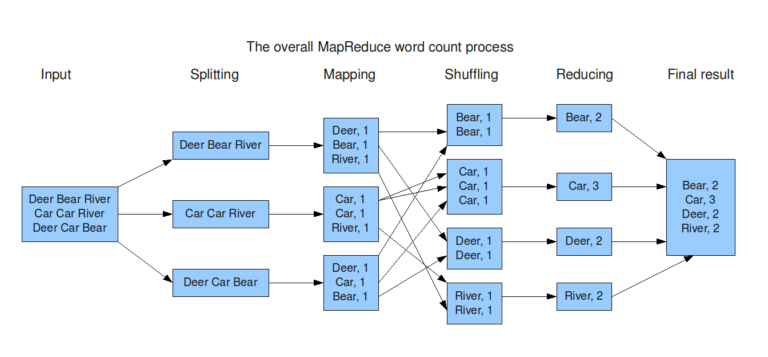
\includegraphics[scale=0.3]{images/ris_01.png}

$http://www.igfasouza.com/blog/$

\end{frame}






\begin{frame}{Существующие, наборы данных, визуализация}

Работа с «грязными» данными: редактирование, форматирование, 
удаление недопустимых значений и дубликатов. 
Агрегирование данных. Основные модели классификации

Рассматривать мы будем  программный продукт Orange3, позволяющий  интерактивно работать с данными.
Для знакомства выполним несколько заданий



\end{frame}

\begin{frame}{Работа с «грязными» данными}

Противоречивость информации;

Пропуски в данных;

Аномальные значения;

Шум;

Ошибки ввода данных. 

\end{frame}



\begin{frame}{Модель алгоритмов, метод обучения.}

Задано множество объектов X, множество допустимых ответов Y. 
Существуют пары <объект,ответ>,  которые будем  называть прецедентами. 
Совокупность  называется обучающей выборкой (training sample).



Задача обучения по прецедентам заключается в том, чтобы по  обучающей выборке 
восстановить зависимость, то есть построить решающую функцию  или алгоритм допускающий эффективную компьютерную 
реализацию.

\end{frame}  

\begin{frame}{Модель алгоритмов, метод обучения.}
В задачах обучения по прецедентам  пара <объект,ответ> 
это не реальные объекты, а лишь доступные данные о них. 
Данные могут быть неточными, поскольку измерения  свойств объектов и ответов обычно
выполняются с погрешностями. 

При это данные могут быть неполными, 
поскольку измеряются не все мыслимые признаки, а лишь физически доступные для измерения.
В результате одному и тому же описанию x могут соответствовать различные объекты и различные ответы. 
\end{frame}  

\begin{frame}{Модель алгоритмов, метод обучения.}

В таком случае   алгоритм или функция описывающие зависмость  не является функцией.
Устранить эту некорректность позволяет вероятностная постановка задачи.
Вместо существования неизвестной целевой зависимости можно считать что 
существует  неизвестное вероятностного распределения на множестве пар объектов и ответов
с плотностью p(x, y), из которого случайно и независимо выбираются  некоторое количество  наблюдений. 
Такие выборки называются простыми или случайными одинаково распределёнными.
Вероятностная постановка задачи считается более общей, так как функциональную зависимость можно 
представить в виде вероятностного распределения $p(x, y) = p(x)p(y|x)$, положив $p(y|x) = \delta(y − y (x))$, где $\delta(z)$ — дельта-функция.

\end{frame}  



\begin{frame}{Основные виды классификаторов машинного обучения.}

Методы машинного обучения можно разделить на 3 основные категории: контролируемое, 
неконтролируемое и подкрепляемое обучение. Контролируемое или обучение с учителем  уже обсуждалось выше.

\end{frame}


\begin{frame}{Основные виды классификаторов машинного обучения.}
Контролируемое обучение полезно в тех случаях, когда свойство (ярлык) доступно для определенного массива данных (обучающего набора), но на данный момент оно отсутствует и должно быть предсказано для других случаев. 
\end{frame}


\begin{frame}{Основные виды классификаторов машинного обучения.}
Неконтролируемое обучение используется для обнаружения неявных отношений в данном немаркированном наборе данных. 

Формально:
Пусть X - множество объектов  - описаний некоторых
объектов. Необходимо найти множество  взаимосвязей этих объектов.
Качество выявления взаимосвязей проверяется некоторой метрикой,
выбранной исходя из решаемой задачи.

\end{frame}


\begin{frame}{Основные виды классификаторов машинного обучения.}


Обучение без учителя используется для решения следующих
типов задач:
1. Задача кластеризации.
2. Поиск правил ассоциации.
3. Сокращение размерности данных.
4. Визуализация данных.

\end{frame}



\begin{frame}{Основные виды классификаторов машинного обучения.}

Под задачей поиска правил ассоциаций подразумевается
выявление в признаковых описаниях объектов (исходных данных)
таких наборов и значений признаков, которые особенно часто
(неслучайно часто) встречаются в исходных данных. Если же
проводить аналогию с первой задачей, то каждое правило в данном
случае может быть представлено как кластер.

\end{frame}


\begin{frame}{Основные виды классификаторов машинного обучения.}


Задача сокращения размерности данных состоит в следующем.
Существует большой (значительно большой) объем признаковых
описаний объектов. Причем, этот объем обуславливается
внушительным количеством измерений признакового пространства.
Необходимо представить те же данные в пространстве меньшей
размерности, при этом минимизировав потери информации.
Группировка по кластерам как раз и будет одним из вариантов
решения проблемы.
\end{frame}


\begin{frame}{Основные виды классификаторов машинного обучения.}


Задача визуализации данных является по сути частным случаем
предыдущей: ее суть – представить исходные данные в отображаемом
пространстве, то есть пространстве размерности 2 или 3.
Как следует из описанного выше, обучение без учителя в какой-
то мере так или иначе сводится к кластеризации. Поэтому для оценки
качества обучения данным способом как правило используют
метрики качества кластеризации. Причем, при их выборе
учитывается, что эти метрики не должны зависеть от исходных

\end{frame}






\begin{frame}{Функция потерь и функционал качества.}

Функция потерь (loss function) — это неотрицательная функция $L (a, x)$,
характеризующая величину ошибки алгоритма a на объекте x. Если $L (a, x) = 0$,
то ответ $a(x)$ называется корректным.



\end{frame}


\begin{frame}{Функция потерь и функционал качества.}
$ L (a, x) = [a(x) + b = y^∗ (x)]$ - индикатор несовпадения с правильным ответом
(обычно применяется в задачах классификации);


$L (a, x) = |a(x) − y ∗ (x)| > \epsilon$  - индикатор существенного отклонения от пра-
вильного ответа, где $\epsilon$ - заданный порог точности.


\end{frame}

\begin{frame}{Функция потерь и функционал качества.}

Вообще, если L принимает только два значения 0 и 1, причём 1 соответствует ошибке,
 то функционал Q называется частотой ошибок алгоритма a на выборке X.

$L (a, x) = |a(x) − y^∗ (x)|$ — величина отклонения от правильного ответа; функ-
ционал Q называется средней ошибкой алгоритма a на выборке X ;

$L (a, x) = (a(x)−y^∗ (x))^2$ — квадрат отклонения от правильного ответа; функци-
онал Q называется средней квадратичной ошибкой алгоритма a на выборке X.

$L w (a, x) = w(x)L (a, x)$ — взвешенная функция потерь, где $w(x)$ — неотрица-
тельная весовая функция, характеризующая степень важности объекта x или
величину потери от ошибки на данном объекте; $L (a, x)$ — некоторая функция
потерь, например, любая из перечисленных выше.


\end{frame}




 
\begin{frame}{Принцип минимизации эмпирического риска.}

Эмпирическим риском называется средняя ошибка алгоритма на обучающей выборке. Метод минимизации эмпирического риска (empirical risk minimization, ERM) наиболее часто применяется для построения алгоритмов обучения. Он состоит в том, чтобы в рамках заданной модели выбрать алгоритм, имеющий минимальное значение средней ошибки на заданной обучающей выборке.

\end{frame}

\begin{frame}{Принцип минимизации эмпирического риска.}
С переобучением метода ERM связано два утверждения, которые на первый взгляд могут показаться парадоксальными.

Утверждение 1. Минимизация эмпирического риска не гарантирует, что вероятность ошибки на тестовых данных будет мала. Легко строится контрпример — абсурдный алгоритм обучения, который минимизирует эмпирический риск до нуля, но при этом абсолютно не способен обучаться. 

\end{frame}

\begin{frame}{Принцип минимизации эмпирического риска.}

Алгоритм состоит в следующем. Получив обучающую выборку, он запоминает её и строит функцию,
 которая сравнивает предъявляемый объект с запомненными обучающими объектами. 
 Если предъявляемый объект в точности совпадает с одним из обучающих, то эта функция 
 выдаёт для него запомненный правильный ответ. Иначе выдаётся произвольный ответ (например, случайный или всегда один и тот же). 
 Эмпирический риск алгоритма равен нулю, однако он не восстанавливает зависимость и не обладает никакой способностью к обобщению.

Вывод: для успешного обучения необходимо не только запоминать, но и обобщать.

\end{frame}

\begin{frame}{Принцип минимизации эмпирического риска.}


 Переобучение появляется именно вследствие минимизации эмпирического риска. Пусть задано конечное множество из D алгоритмов, 
которые допускают ошибки независимо и с одинаковой вероятностью. Число ошибок любого из этих алгоритмов 
на заданной обучающей выборке подчиняется одному и тому же биномиальному распределению.
 Минимум эмпирического риска — это случайная величина, равная минимуму из D 
 независимых одинаково распределённых биномиальных случайных величин. 
 Её ожидаемое значение уменьшается с ростом D. Соотвественно, с ростом D увеличивается 
 переобученность — разность вероятности ошибки и частоты ошибок на обучении.
 
\end{frame}

\begin{frame}{Принцип минимизации эмпирического риска.}

В данном модельном примере легко построить доверительный интервал переобученности, так как функция распределения минимума известна.
 Однако в реальной ситуации алгоритмы имеют различные вероятности ошибок, не являются независимыми,
  а множество алгоритмов, из которого выбирается лучший, может быть бесконечным.
   По этим причинам вывод количественных оценок переобученности является сложной задачей,
    которой занимается теория вычислительного обучения. До сих пор остаётся открытой 
    проблема сильной завышенности верхних оценок вероятности переобучения.
    
\end{frame}

\begin{frame}{Принцип минимизации эмпирического риска.}

Утверждение 3. Переобучение связано с избыточной сложностью используемой модели. Всегда существует оптимальное значение сложности модели, при котором переобучение минимально. 

\end{frame}

\begin{frame}{Обобщающая способность}

Обобщающая способность (generalization ability, generalization performance). Говорят, что алгоритм обучения обладает способностью к обобщению, если вероятность ошибки на тестовой выборке достаточно мала или хотя бы предсказуема, то есть не сильно отличается от ошибки на обучающей выборке. Обобщающая способность тесно связана с понятиями переобучения и недообучения.
\end{frame}

\begin{frame}{Обобщающая способность.}

Переобучение, переподгонка (overtraining, overfitting) — нежелательное явление, возникающее при решении задач обучения по прецедентам, когда вероятность ошибки обученного алгоритма на объектах тестовой выборки оказывается существенно выше, чем средняя ошибка на обучающей выборке. Переобучение возникает при использовании избыточно сложных моделей.

Недообучение — нежелательное явление, возникающее при решении задач обучения по прецедентам, когда алгоритм обучения не обеспечивает достаточно малой величины средней ошибки на обучающей выборке. Недообучение возникает при использовании недостаточно сложных моделей. 

\end{frame}

\begin{frame}{Скользящий контроль}

Скользящий контроль или кросс-проверка или кросс-валидация (cross-validation, CV) — процедура эмпирического оценивания обобщающей способности алгоритмов, 
обучаемых по прецедентам.

Фиксируется некоторое множество разбиений исходной выборки на две подвыборки: обучающую и контрольную. Для каждого разбиения выполняется 
настройка алгоритма по обучающей подвыборке, затем оценивается его средняя ошибка на объектах контрольной подвыборки.
Оценкой скользящего контроля называется средняя по всем разбиениям величина ошибки на контрольных подвыборках.

\end{frame}

\begin{frame}{Скользящий контроль}

Если выборка независима, то средняя ошибка скользящего контроля даёт несмещённую оценку вероятности ошибки. 
Это выгодно отличает её от средней ошибки на обучающей выборке, которая может оказаться смещённой 
(оптимистически заниженной) оценкой вероятности ошибки, что связано с явлением переобучения.

Скользящий контроль является стандартной методикой тестирования и сравнения алгоритмов классификации, регрессии и прогнозирования. 

\end{frame}


\begin{frame}{Основные виды}

\end{frame}




\begin{frame}{Логистическая регрессия}
Логистическая регрессия представляет собой мощный статистический способ прогнозирования вероятности возникновения 
некоторого события с одной или несколькими независимыми переменными.
 Логистическая регрессия определяет степень зависимости между категориальной зависимой и одной или несколькими 
 независимыми переменными путем использования логистической функции, являющейся аккумулятивным логистическим распределением. 

\end{frame}




\begin{frame}{Логистическая регрессия.Алгоритм}
Линейная регрессионная модель не всегда способна качественно предсказывать значения зависимой переменной. Выбирая для построения модели линейное уравнение, мы естественным 
образом не накладываем никаких ограничений на значения зависимой переменной. А такие ограничения могут быть существенными.

Например, при проектировании оптимальной длины шахты лифта в новом здании необходимо учесть, что эта длина не может превышать высоту здания вообще.
\end{frame}


\begin{frame}{Логистическая регрессия.Алгоритм}

Линейная регрессионная модель может дать результаты, несовместимые с реальностью. С целью решения данных проблем полезно изменить 
вид уравнения регрессии и подстроить его для решения конкретной задачи.

Вообще, логит регрессионная модель предназначена для решения задач предсказания 
значения непрерывной зависимой переменной, при условии, что эта зависимая переменная 
может принимать значения на интервале от 0 до 1.
\end{frame}

\begin{frame}{Логистическая регрессия. Сигмоид}

Сигмоид — это гладкая монотонная возрастающая нелинейная функция,
 имеющая форму буквы «S», которая часто применяется для «приближения» 
 значений некоторой величины к нулю и единице


$$  y=a_0 + a_1x_1+ a_2x_2 ...+a_nx_n $$

$$ f(y) = \frac{1}{1 + e^{-y}}$$



\end{frame}



\begin{frame}{Логистическая регрессия.Применение}

Данный алгоритм может быть использован для:
    \begin{itemize}

  \item оценки компартмента предприятия с использованием косвенных данных связи с другими предприятиями в прошлом объемы по типам продукции, регион и т.п.;
  \item измерении показателей успешности  тех или иных мер;
  \item предсказании доходов с определенного продукта;
    \end{itemize}
    

\end{frame}





\begin{frame}{Дерево принятия решений}

Дерево принятия решений — средство поддержки принятия решений, которое использует 
древовидный граф или модель принятия решений, а также возможные последствия их работы, 
включая вероятность наступления события, затраты ресурсов и полезность. 

\end{frame}


\begin{frame}{Дерево приннятия решения}

Деревья принятия решений и случайные леса

Один из самых распространeнных алгоритмов машинного обучения.
 Используется в статистике и анализе данных для прогнозных моделей. 
 Структура представляет собой "листья" и "ветки". 
 На "ветках" дерева решения записаны атрибуты, 
 от которых зависит целевая функция, в "листьях” записаны значения целевой функции, 
 а в остальных узлах – атрибуты, по которым различаются случаи.

\end{frame}


\begin{frame}{Дерево приннятия решения. Алгоритм}


Чтобы классифицировать новый случай, надо спуститься по дереву до листа и выдать соответствующее значение. 
Цель состоит в том, чтобы создать модель, которая предсказывает значение целевой 
переменной на основе нескольких входных переменных. Осуществляется перебор  столбцов.
\end{frame}

\begin{frame}{Дерево принятия решения. Пример}


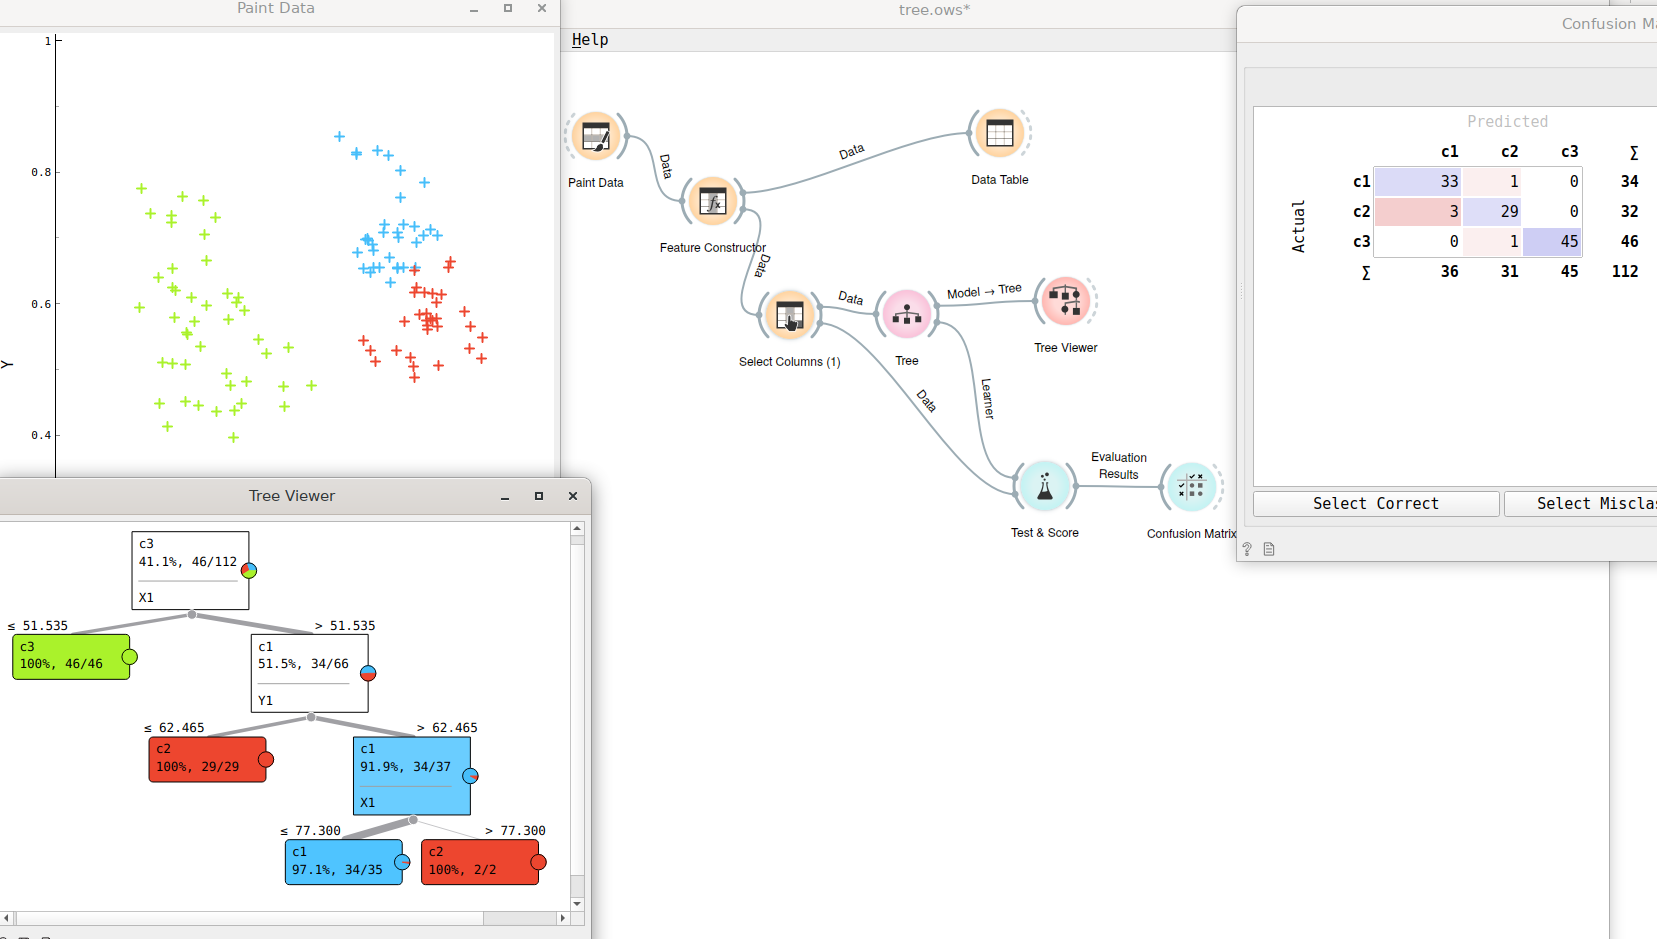
\includegraphics[scale=0.2]{images/task08_01.png}

\end{frame}


\begin{frame}{Дерево принятия решения. Пояснения}


\begin{textblock*}{120mm}(15mm,15mm)
 

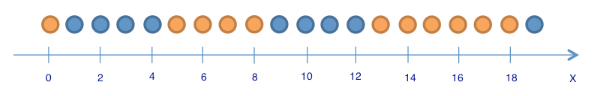
\includegraphics[scale=0.4]{images/ris_02.png}

\end{textblock*} 


\begin{textblock*}{90mm}(15mm,35mm)
Если мы наудачу вытащили шарик, 
то он с вероятностью $ p_1=\frac{9}{20} $ будет синим и с вероятностью $ p_2=\frac{11}{20} $ – желтым. 
Значит, энтропия состояния  $S_0=-\frac{9}{20}log_2{\frac{9}{20}}-\frac{11}{20}log_2{\frac{11}{20}} \approx 1$

Само это значение пока ни о чем нам не говорит. 
Как изменится энтропия, если разбить шарики на две группы – с координатой меньше либо равной 12 и больше 12?

$https://www.pvsm.ru/python/249240$
\end{textblock*} 



\end{frame}


\begin{frame}{Дерево принятия решения. Пояснения}

\begin{textblock*}{120mm}(15mm,15mm)

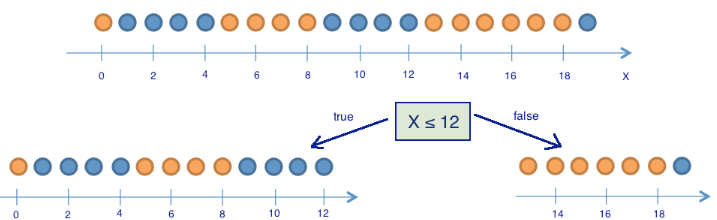
\includegraphics[scale=0.35]{images/ris_03.png}

\end{textblock*} 

\begin{textblock*}{90mm}(15mm,50mm)
В левой группе оказалось 13 шаров, из которых 8 синих и 5 желтых. 
Энтропия этой группы равна
 $S_1=-\frac{5}{13}log_2{\frac{5}{13}}-\frac{8}{13}log_2{\frac{8}{13}} \approx 0.96$. 
В правой группе оказалось 7 шаров, из которых 1 синий и 6 желтых. 
Энтропия правой группы равна 
$S_2=-\frac{1}{7}log_2{\frac{1}{7}}-\frac{6}{7}log_2{\frac{6}{7}} \approx 0.6$

$https://www.pvsm.ru/python/249240$
\end{textblock*} 


\end{frame}

\begin{frame}{Метод опорных векторов (SVM) }
Метод опорных векторов (SVM) — это набор алгоритмов, использующихся для задач классификации и регрессионного анализа. 
Учитывая, что в N-мерном пространстве каждый объект принадлежит одному из двух классов, SVM генерирует (N-1)-мерную 
гиперплоскость с целью разделения этих точек на 2 группы. Это как если бы вы на бумаге изобразили точки двух разных 
типов, которые можно линейно разделить. Помимо того, что метод выполняет сепарацию объектов, SVM подбирает 
гиперплоскость так, чтобы та характеризовалась максимальным удалением от ближайшего элемента каждой из групп.
\end{frame}


\begin{frame}{SVM. Пример}


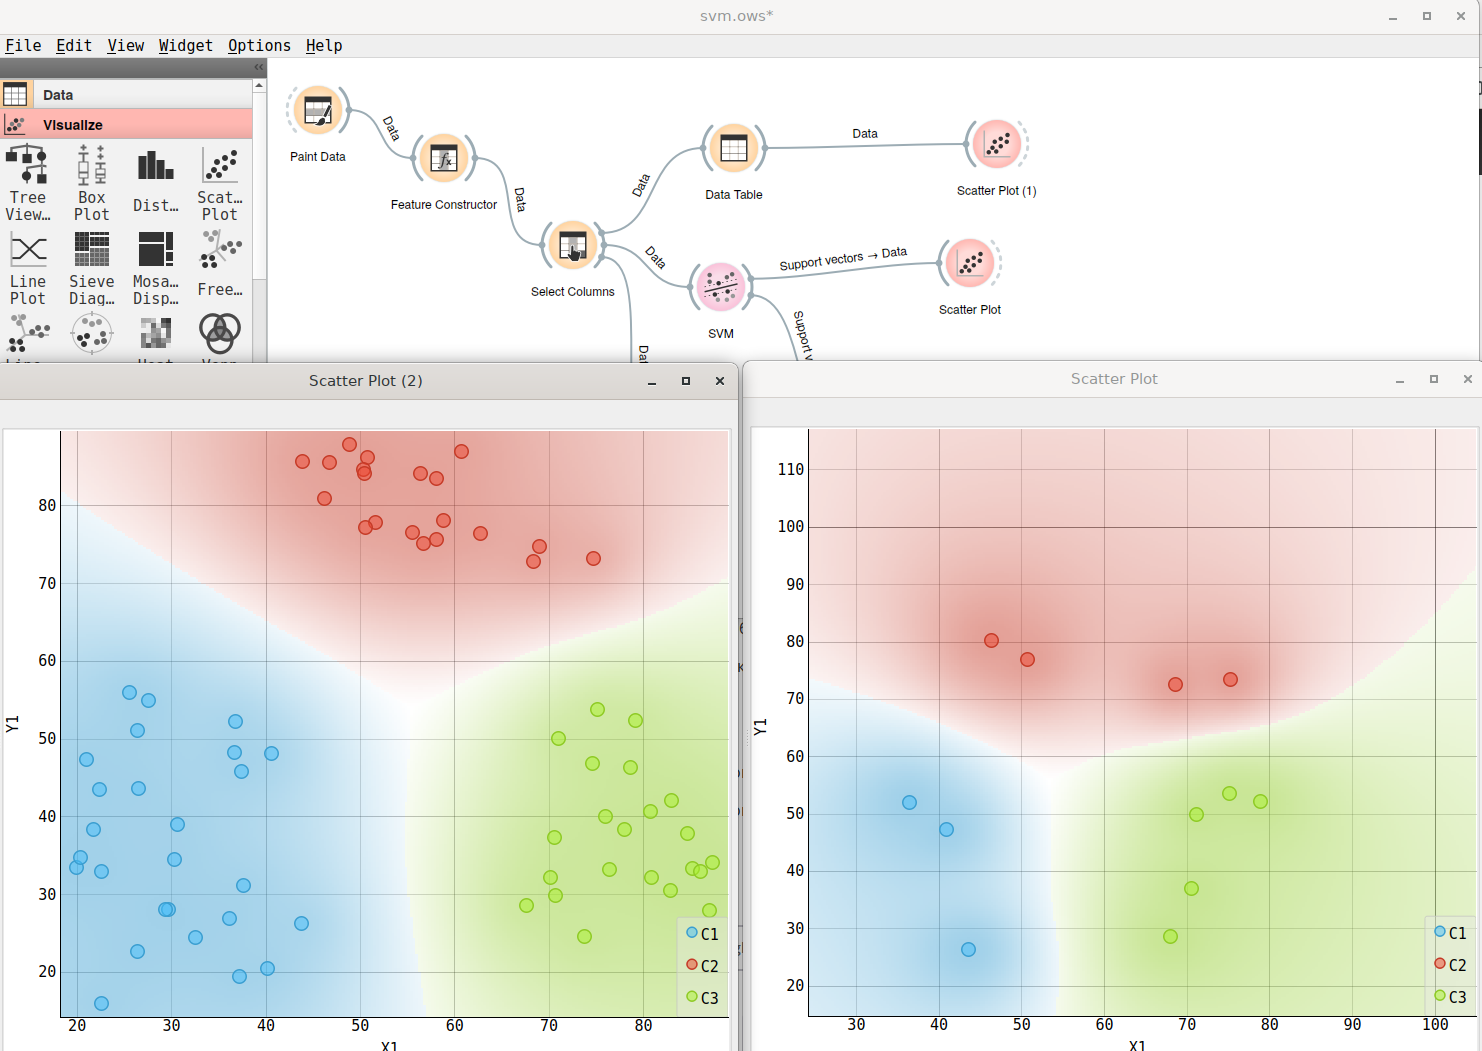
\includegraphics[scale=0.2]{images/task09_01.png}

\end{frame}

\begin{frame}{Метод ансамблей}

Метод ансамблей основан на обучающих алгоритмах, которые формируют множество классификаторов, а затем сегментируют 
новые точки данных, отталкиваясь от голосования или усреднения. 
Оригинальный метод ансамблей — не что иное, как Байесовское усреднение, но более поздние алгоритмы включают исправления ошибок выходного кодирования, бэггинг (bagging) и бустинг (boosting). 
\end{frame}


\begin{frame}{Метод ансамблей}

Бустинг направлен на превращение слабых моделей в сильные путем построения ансамбля классификаторов. 
Бэггинг также агрегирует усовершенствованные классификаторы, но используется при этом параллельное обучение 
базовых классификаторов. Бэггинг — улучшающее объединение, а бустинг — улучшающее пересечение.
\end{frame}


\begin{frame}{Random Forest}
Метод случайного леса (Random Forest) представляет собой дальнейшее улучшение бэггинга деревьев решений, 
которое заключается в устранении корреляции между деревьями. Как и в случае с бэггингом,
 мы строим несколько сотен деревьев решений по обучающим бутстреп-выборкам. 
 Однако на каждой итерации построения дерева случайным образом выбирается m из p подлежащих рассмотрению предикторов и разбиение разрешается выполнять только по одной из m этих переменных.
\end{frame}

\begin{frame}{Random Forest}
Смысл этой процедуры, оказавшейся весьма эффективной для повышения качества получаемых решений, заключается в том, что с вероятностью (p−m)/p
блокируется какой-нибудь потенциально доминирующий предиктор, стремящийся войти в каждое дерево. Если доминирование таких предикторов разрешить, то все деревья в итоге будут очень похожи друг на друга, а получаемые на их основе предсказания будут сильно коррелировать и снижение дисперсии будет не столь очевидным. Благодаря блокированию доминантов, другие предикторы получат свой шанс, и вариация деревьев возрастает.
\end{frame}

\begin{frame}{Random Forest}
Выбор малого значения m при построении случайного леса обычно будет полезным при наличии большого числа коррелирующих предикторов. Естественно, если случайный лес строится с использованием m=p, то вся процедура сводится к простому бэггингу.
\end{frame}


  
\end{document}
